\documentclass[11pt]{article}
\usepackage[utf8]{inputenc} % Para caracteres en espa�ol
\usepackage{amsmath,amsthm,amsfonts,amssymb,amscd}
\usepackage{multirow,booktabs}
\usepackage[table]{xcolor}
\usepackage{fullpage}
\usepackage{lastpage}
\usepackage{enumitem}
\usepackage{multicol}
\usepackage{fancyhdr}
\usepackage{mathrsfs}
\usepackage{wrapfig}
\usepackage{setspace}
\usepackage{esvect}
\usepackage{calc}
\usepackage{multicol}
\usepackage{cancel}
\usepackage{graphicx}
\graphicspath{ {pictures/} }
\usepackage[retainorgcmds]{IEEEtrantools}
\usepackage[margin=3cm]{geometry}
\usepackage{amsmath}
\newlength{\tabcont}
\setlength{\parindent}{0.0in}
\setlength{\parskip}{0.05in}
\usepackage{empheq}
\usepackage{framed}
\usepackage[most]{tcolorbox}
\usepackage{xcolor}
\colorlet{shadecolor}{orange!15}
\parindent 0in
\parskip 12pt
\geometry{margin=1in, headsep=0.25in}
\theoremstyle{definition}
\newtheorem{defn}{Definition}
\newtheorem{reg}{Rule}
\newtheorem{exer}{Exercise}
\newtheorem{note}{Note}
\newcommand{\volume}{{\ooalign{\hfil$V$\hfil\cr\kern0.08em--\hfil\cr}}}
\newcommand{\parr}{\mathbin{\|}} % Parralel Symbol
\begin{document}
\setcounter{section}{2}
\setcounter{page}{23}
\setcounter{equation}{49}

 \pagestyle{fancy}
\fancyhf{}
\rhead{Section 2: Electromagnetics}
\rfoot{Page \thepage}
\thispagestyle{empty}


\begin{center}
{\LARGE \bf Section 2: Electromagnetics}\\
{\large AE435}\\
Spring 2018
\end{center}
In this section, we will review the basics of charge, electricity, magnetism, and Maxwell equations.
\vspace{25mm}
\section{Magnetostatics}
\begin{center}
"Charge in motion creates a magnetic field"
\end{center}
\tableofcontents
\newpage
\subsection{Electric Current}
\begin{shaded}
\textbf{Current} \newline
\begin{equation}
J \equiv \frac{\partial Q}{\partial t} \qquad \bigg[\frac{c}{s}\bigg] = \big[A\big] = \text{Amps}
\end{equation}
\end{shaded}
We'll use J, although sometimes we see I used for current. Currents can flow in a range of media: metals, semiconductors, fluids, gases and plasmas.

\textbf{METALS}
\newline
In metals, there are fixed ionic cores with bound inner ions:
\begin{center}
\vfill
\textbf{Figure 10}
\end{center}
Outer valence electrons get freely traded from ion to ion in response to electric fields. In other words, say we put  10 electrons in one end of a wire and we get 10 electrons out the other end. Those won't be the same 10 electrons we put in though.

\textbf{GASES AND PLASMAS}
\newline
In gases and plasmas, both electrons AND ions move:
\begin{center}
\vfill
\textbf{Figure 11}
\end{center}
\begin{itemize}
\item Most of the conduction is by electrons, because they're much lighter.
\item In thermal motion, both ions and electrons are as likely to cross plane in one direction as another, so no net current.
\item Under electric field, drift velocity of species (ions toward cathode, electrons toward anode) gives rise to current.
\end{itemize}
\newpage
\subsection{Current Density}
Consider flux of particles through surface element dS:
\begin{center}
\vfill
\textbf{Figure 12}
\end{center}
Since particle with charge q crossing dS carries incremental current $q \, \vv{v} \cdot \hat{n}$. For N particles per unit volume, current crossing dS is then:
\begin{equation*}
\begin{aligned}
\mathrm{d}J = N \, q \, \vv{v} \cdot \hat{n} \, \mathrm{d}S
\end{aligned}
\end{equation*}
For multiple species, sum over all:
\begin{equation*}
\begin{aligned}
\mathrm{d}J = \sum_i N_i \, q_i \, \vv{v}_i \cdot \hat{n} \, \mathrm{d}S
\end{aligned}
\end{equation*}
Define current density as a vector current per unit area:
\begin{shaded}
\textbf{Current Density} \newline
\begin{equation}
\vv{j} = \sum_i N_i \, q_i \, \vv{v}_i \qquad \bigg[\frac{A}{m^2}\bigg]
\end{equation}
\end{shaded}
So, the total current across a surface S is:
\begin{shaded}
\textbf{Total Current Across a Surface} \newline
\begin{equation}
J = \int_S \vv{j} \cdot \hat{n} \, \mathrm{d}S
\end{equation}
\end{shaded}
\newpage
\subsection{Continuity}
Consider volume V enclosed by surface S, within a current density field
\newline
\newline
Current crossing in or out of V through S is:
\newline
\newline
Note positive current is into the volume.
\newline
\newline
We also know from the definition of current (2.50), and
from definition of volume charge density, and for a steady
control volume:
\newline
\newline
Combining Eqns. (2.54) (2.53)
\newline
\newline
This must be true for an arbitrary volume, so the
integrand must vanish at every point, giving:
\newpage
\subsection{Ohm's Law}
Experiments show that
\newline
\newline
Where the conductivity has units of Siemens/m. In
common conductors (metals, electrolytes, unmagnetized
plasmas)
 a constant. These are called linear media
or ohmic media. If you take the reciprocal of the
conductivity, you get the resistivity,
\newline
\newline
which has units of Ohm-m, and is tabulated in lots of
easy-to-find places (the CRC Handbook, multiple places
on the web).
\newline
\newline
For steady currents, . By continuity
then:
\newline
\newline
or substituting in conductivity:
\newline
\newline
For homogeneous media (constant over space):
which for electrostatic fields is just Laplace's Eqn.
\newline
\newline
Given boundary conditions of or at
surfaces of a medium, can solve for in the
medium.
\newpage
\subsection{Magnetic Field}
Recall our description of force on a charge, Coulomb's
Law, from section II.A.1.
\newline
\newline
Again, look at a TWO-PARTICLE model.
\newline
\newline
The force on q due to q1 is Eqn. (2.1).
\newline
\newline
But what if the charges are moving? Let q move at a
velocity and q1 move at a velocity . In this case,
there's now another force on q due to q1 . This force is the
magnetic force.
\newline
\newline
where is the permeability of free space. In SI units,
the constant of proportionality is defined as:
\newline
\newline
By grouping terms relating to the field charge q1 , we can
define a vector field that represents the force on the test
charge q moving at velocity . So that:
\newline
\newline
where
\newline
\newline
This vector field is the magnetic induction a.k.a.
magnetic field intensity, and has SI units Tesla.
\newline
\newline
Total force on test charge q is then Electric AND
Magnetic forces, which is called the Lorentz force.
\newline
\newline
Work done by a stationary magnetic field?
\newline
\newline
A stationary magnetic field cannot do work/accelerate a
fluid/particle/charge.
\newpage
\subsection{Forces on Conductors}
Consider a conducting circuit immersed in a B-field.
Charges with a number density F move at a velocity
along a wire section with a cross-sectional area
A.
\newline
\newline
The total charge in this section is:
\newline
\newline
And so the total magnetic force on this section is:
\newline
\newline
Since the current runs along the wire, , then
we can swap locations in the vector equation:
\newline
\newline
Recall that the current density magnitude
(2.51) , and that total current (2.52), then:
\newline
\newline
Integrating over the entire circuit, the total magnetic
force on the circuit is:
\newline
\newline

\newpage
\subsection{Biot-Savart Law}
\newpage
%%%%%%%%%%%%%%%%%%%%%%%%%%%%%%%%%%%%%%%%%%%%%%%%%%%%%%%%
%%%%%%%%%%%%%%                         BASIC TEMPLATES                                %%%%%%%%%%%%%%
%%%%%%%%%%%%%%%%%%%%%%%%%%%%%%%%%%%%%%%%%%%%%%%%%%%%%%%%
\section{Basic Templates}
% Basic Note Guides
\begin{note} \textbf{This is how you make numbered notes}\end{note}
\begin{exer} \textbf{This is how you make numbered exercises}\end{exer}
\begin{defn} \textbf{This is how you make numbered definitions}\end{defn}
\begin{reg} \textbf{This is how you make numbered rules}\end{reg}

%Shaded Equations + Explainer
\begin{shaded}
\textbf{Equation Name} \newline
\begin{equation*}
y = mx + b
\end{equation*}
Where:
\begin{equation*}
\begin{split}
variable1 &= \text{Description} \\
variable2 &= \text{Description} \\
\end{split}
\end{equation*}
\end{shaded}

%Insert Photo
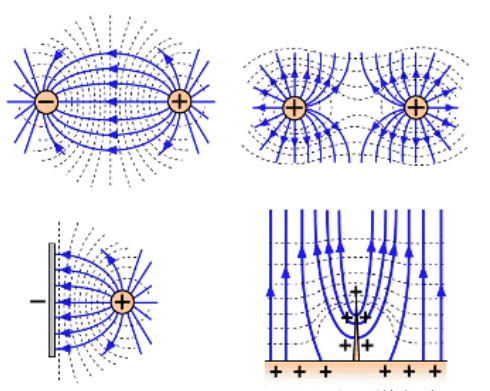
\includegraphics[scale=0.75]{1.png}

\end{document}